%\dropchapter{0.4in}
\chapter{chapter 3} \label{chp:labelTitle}
%\epigraphhead[70]{\epigraph{\textit{If I could remember the names of all these particles, I'd be a botanist.}}{Enrico Fermi}}
%\undodrop

An accurate understanding of simulated events and their reconstruction is crucial for a thorough understanding of the collected data. Hence event generators such as $\Madgraph$, $\Pythia$ and $\Herwig$ play the role of hadron colliders and allow some improvement of analyzing power by using an efficient background and signal discriminator.

\section{QCD for hadron colliders} \label{sec::QCDHadron}

The event generation process in hadron colliders is arduous due to QCD activity in a widespread energy range. The phenomena of interest studied by the LHC consist of momentum transfers in a range between $50$ $\GeV$ and $5$ $\TeV$, however, the initial partons responsible for these collisions are protons with a mass of barely $0.938$ $\GeV$. The first energy range results in a tiny QCD coupling ($\alpS$) and perturbation theory can be assumed to be valid, while the energy range of the incoming partons is too low for perturbation theory to hold. Therefore throughout the consecutive steps of the event generation process some aspects can be derived exactly from the QCD Lagrangian while others are expressed through phenomenological non-perturbative models. An overview of this process is depicted in Figure~\ref{fig::EvtShower}, which will be discussed further in this section and are depicted in Figure~\ref{fig::EvtShower},% without losing all predictive power.
%\textit{Is there still a part which is described by perturbative QCD? Everything is approximate no?}  --> Perturbative part is the HARD scattering!

\begin{figure}[htb]
 \centering
 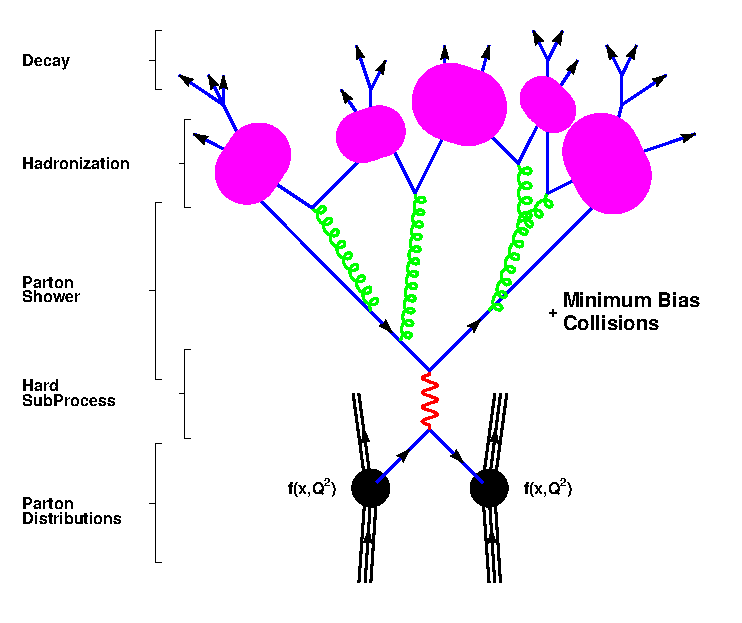
\includegraphics[width = 0.8 \textwidth]{Chapters/Chapter3/Figures/f_shg_event.eps}
 \caption{Schematical overview of the consecutive steps of the event generation process.}  \label{fig::EvtShower}
\end{figure}

\begin{myindentpar}
  \begin{description}
    \item[Parton Distribution Functions] \hfill \\
      In proton-proton collisions both incoming protons can be seen as a collection of partons whose momentum fraction $x$ within the hadron is parametrized by the so-called parton distribution functions.
    \item[Hard scattering (or factorization?)] \hfill \\
      The perturbative process when collision of two partons or gluons creates high-energetic particles is defined as hard scattering, and can be calculated by a factorized product of short-and long-distance processes as discussed in Section~\ref{sec::HardScattering}.
    \item[Parton shower (or is this factorization??)] \hfill \\
      This phase of the event generation process includes the approximate higher-order corrections induced by emission of additional gluon and/or quarks, as will be explained in detail in Section~\ref{sec::PS}. Depending whether this radiation originates from the incoming or the outgoing partons this is called Initial State Radiation (ISR) or Final State Radiation (FSR), respectively.
    \item[Hadronisation] \hfill \\
      Due to color confinement the collection of (receding) post-shower partons has to combine into experimentally observable color-neutral hadrons. This process, called hadronisation, is described by QCD-inspired phenomenological models as will be discussed in Section~\ref{sec::Hadronisation}.
    %\item[Underlying event (why is this a separate item? Doesn't show up in the schematical overview ...)] \hfill \\
  \end{description}
\end{myindentpar}

\subsection{Hard Scattering (=? Jet Fragmentation)} \label{sec::HardScattering}
Due to the internal structure of the protons, the inclusive cross section $\sigma_{h_{1}h_{2} \rightarrow X}$ cannot be calculated exactly from first principles. It has to be factorized in terms of the partonic scattering cross section $\hat{\sigma}_{ab \rightarrow X}$ and the parton distribution functions $f_{a}^{h}$. Therefore, within the collinear limit~\cite{ColLimit}, the inclusive cross section for $X$-production can be written as:
%Since the hard scattering interaction occurs between two partons present in the proton, it probes the energy scale far below the mass range of the proton. In this region perturbative QCD is valid and the cross-section can be calculated from first principles (not completely true, the PDF's cannot be calculated from first principles since it concerns small momentum transfers!!) REMARK: LOW ENERGY SCALE MEANS NO PQCD!!.\\
%Within collinear factorization the cross-section of such an hard interacting event can be seen as a convolution between the partonic cross section $\hat{\sigma}$ and the long-scale parton distribution functions (PDF's) which represent the flux of the partons within the proton. (\textit{BETTER LAST SENTENCE!})\\
%The inclusive cross section of creating the final state $X$ from the hadrons $h_{1}$,$h_{2}$ can be written in terms of the partonic cross section $\hat{\sigma}_{ab \rightarrow X}$: (\textit{Still not much better.}
\\ \textit{Should check whether there is a difference between $\hat{\sigma}_{ab \rightarrow X}$ and $\hat{\sigma}(\Phi_{ab \rightarrow X},\mu^{2}_{F})$??}
\begin{equation} \label{eq::HSXS}
 \sigma_{h_{1}h_{2} \rightarrow X} =\sum_{a,b \in \{q,g\} } \int dx_{a} \int dx_{b} f_{a}^{h_{1}}(x_{a},\mu^{2}_{F}) f_{b}^{h_{2}}(x_{b},\mu^{2}_{F}) \int d\Phi_{ab \rightarrow X} \dfrac{d\hat{\sigma}(\Phi_{ab \rightarrow X},\mu^{2}_{F})}{d\Phi_{ab \rightarrow X}}
\end{equation}
As Equation~(\ref{eq::HSXS}) suggests, the hadronic cross section is actually a convolution of a perturbatively short-distance part $\hat{\sigma}_{ab \rightarrow X}$, calculable from Matrix Elements, and an approximately long-distance part, represented by the parton distribution functions (PDF). The PDF $f_{a}^{h}(x_{a},\mu_{F})$ symbolizes the probability of encountering a parton $a$ with momentum fraction $x_a$ within the hadron $h$ at the energy scale $\mu_{F}$. This factorization scale $\mu_{F}$ represents the transition from the short-distance process to the long-distance one.\\
\textit{Should the terms of the second integrand be mentioned specifically??}\\
\\
\textit{What else can/should be written about this subject ...?}\\
\textit{Elaborate on LO vs NLO difference maybe ...}\\
Leading Order (LO) calculations are fully automated and included explicitely in the general-purpose Monte Carlo event generators. However, since rather recently, in order to improve accuracy and predictive power much effort has been maid to obtain Next-to-Leading-Order (NLO) matrix element calculations.\\
\textit{Check which event generators actually have this NLO calculations and whether this is only for some matrix elements.}\\
\textit{Maybe briefly explain difference between LO and NLO, or is this already done in another chapter?}\\
\\
\textit{Also add a paragraph that explains which event generators are used in this thesis and what their main differences are.}\\
\\
\textit{Maybe brief discussion about LHAPDF and the used PDF set in this thesis (or does this only come after the Parton Shower part has been explained?)}

\subsection{Parton shower} \label{sec::PS}
The hard scattering interaction simulated by the event generator occurs at high energy scales and should (\textit{nevertheless}) still be connected to the lower scale where confinement into hadrons takes place. The communication between these two distinct energy scales is described by the Parton Shower (PS) formalism, a phenomena extractable from QCD's first principles.
As charged particles (\textit{or only electrons?)} radiate Brehmstrahlung in QED, QCD partons are susceptible to the emission of gluon radiation. Moreover, due to the non-Abelian nature of QCD, gluon branching $g$ $\rightarrow$ $gg$ is also permitted.\\
%\\
%\textit{Does the soft and collinear follows from the processes or from the fact that these result in divergences? I think the latter ...}\\
%Since both processes correspond to soft and collinear QCD radiation, parton branching cannot be described by a perturbative calculation and will results in soft divergences. %This iterative splitting (is described by a Markov chain and) reduces the transverse momentum of the original parton until the QCD confinement limit is reached.\\
\\
The objective of the PS formalism is decomposing this complex process into an iterative parton branching procedure. This sequential splitting lowers stepwize the transverse momentum of the contributing partons until the QCD confinement limit is reached and gives rise to a parton cascade. The basic ingredient of this factorization is the probability distribution of a single parton emission from a hard interaction, which is represented by the DGLAP evolution equations:
\begin{equation}\label{eq::PSProb_NoSudakov}
 d\mathcal{P}_{ba} = \dfrac{\sigma_{ME}}{\sigma_{0}} = \dfrac{\alpha_{S}}{2\pi} \frac{4}{3} \frac{dQ^{2}}{Q^{2}} P_{ba}(z)dz
\end{equation}
with $Q^{2}$ \textit{blabla}, $\sigma_{ME}$ the cross section of the hard interaction calculable from Matrix Elements, $\sigma_{0}$ the cross section without parton emission and $z$ the energy fraction carried away by the emitted parton in the hard interaction (\textit{with all divergences and sudakov, can one really call this a 'hard' interaction?}).\\
The form functions $P_{ba}$ are the Alterelli-Parisi splitting functions which describe the splitting of the parton $b$ into parton $a$. They are given by (\textit{Use something else than eqnarray!!}):
\begin{eqnarray}
 & P_{qq}(z) = \dfrac{4}{3} \dfrac{1+z^{2}}{1-z} & P_{qg}(z) = \dfrac{4}{3} \frac{1+(1-z)^{2}}{z} \\
 & P_{gq}(z) = \dfrac{n_{f}}{2} (z^{2} + (1-z)^{2}) & P_{gg}(z) = 3 \dfrac{z^{4}+1+(1-z)^{4}}{z(1-z)}
\end{eqnarray}
where $n_{f}$ represents the number of quark flavours.

The probability for a parton branching $b$ $\rightarrow$ $a$, represented by $\mathcal{P}_{ba}$, diverges in the limit of soft-gluon radiation, dependent on the numerator of the splitting function $z$ $\rightarrow$ $0$ and/or $z$ $\rightarrow$ $1$, and in the limit of collinear parton radiation, $Q^{2}$ $\rightarrow$ $0$.
%$z$ $\rightarrow$ $0$ and $Q^{2}$ $\rightarrow$ $0$, corresponding to soft gluon radiation and collinear parton radiation respectively. 
Both divergences are regulated by introducing a cut-off scale $Q_{0}$ for the parton shower iteration at about $1$ $\GeV$. In the occurence of soft-quark branching (\textit{Why is this still allowed, even after the cut-off is applied? (or is soft quark still larger than 1 GeV?})), the parton branching probability $\mathcal{P}_{ba}$ exceeds unity which would violate the total conservation of probability. This conservation is ensured by including a Sudakov form factor which represents the probability of a parton not to undergo a branching. Hence Equation~(\ref{eq::PSProb_NoSudakov}) should be multiplied by this Sudakov factor and reformulated as:
\begin{equation}
 d\mathcal{P}_{ba} = \dfrac{\alpha_{S}}{2\pi} \dfrac{4}{3} \dfrac{dQ^{2}}{Q^{2}} P_{ba}(z)dz ~ \exp \left\lbrace - \int_{Q_{0}^{2}}^{Q^{2}} \dfrac{dQ^{'2}}{Q^{'2}} \dfrac{\alpha_{S}}{2\pi} \int dz^{'} P_{ba}(z^{'})  \right\rbrace
\end{equation}
%\\
%\textit{$P_{ba}$ can be easily translated to $P_{b \rightarrow a+c}$ by applying the allowed emissions.\\
%qq corresponds to q $\rightarrow$ q which can only be accompanied by gluon radiation hence $P_{qq}$ = $P_{q \rightarrow q g}$ in the definition used above. (check papers for rest)}\\
%\\
%\textit{Such higher order corrections occur in processes where a soft gluon is emitted or when a gluon or light quark splits into two almost collinear partons (NOT OWN WORDS)\\
%Only here does the Sudakov Form Factor and DGLAP equations enter the picture. So they describe the non-perturbative corrections to the hard interaction cross section caused by the soft and collinear splitting of the initial and final state partons.}

The above parton shower algorithm is applicable for both initial state radiation (ISR) and final state radiation (FSR) since the branching probabilities are similar in both cases. However the actual implementation in the Monte Carlo event generators is performed in an entirely different way. This because the parton branching significantly reduces the energy of the initial partons and therefore the possibility to produce the hard process of interest, such as top-quark pair production. 
%In order to avoid the generation of billions of events and keeping only a couple relevant ones, the Monte Carlo event generators employ a backward method. 
Hence the Monte Carlo event generators employ a backward method, meaning they start from the desired hard interaction and surround the initial partons with additional radiation afterwards.

\subsubsection{Combine hard scattering with parton showering}
\textit{Is this also relevant for LO calculations?}\\
\textit{Is only matching used or also merging? (Seems to be applied in HERWIG)}\\

\textit{At leading order correct matching between the produced jets and the original partons asked during the hard interaction is also important. This because additional hard gluon radiation in a X+parton interaction results in the same pattern as the hard interaction of a X+2-parton event. At LO, there are two existing methods which can be used in order to avoid double counting: CKKW and MLM. The latter one, MLM named after M.L. Mangano, is the easier of the two and currently implemented in $ALPGEN$ for use with both $\Herwig$ and $\Pythia$.\\
At next-to-leading order the situation is a bit more complex and two different methods have been developed, $MC@NLO$ and $Powheg$. The former one has a wide range of processes available but can only be used in combination with $HERWIG$. However since recently, effort has been made to also combine the $MC@NLO$ approach with $\Pythia$ and $HERWIG++$. This in contrast to the latter one, which can be intertwined with both $HERWIG$ and $PYTHIA$ but is only recently catching up in the number of available processes.}\\

\textit{What should exactly be discussed?}
The current progress in calculating NLO hard cross section implies a profound understanding and description of the matching between the hard scattering and the parton shower. This is necessary in order to avoid double-counting.

%\subsubsection{Initial State Radiation (ISR)}
%The probability for the incoming partons in the parton bunch to radiate is similar to the branching probability of the partons produced by the hard scattering. Therefore exactly the same formulas and theory can be applied to the radiation of the inital-state partons. However there is an important difference between the initial-state radiation in reality and the implementation in the Monte Carlo event generators. This because the high branching probability significantly reduces the energy of the initial partons and hence the possibility to maintain sufficient energy to produce the hard process of interest, such as top-quark pair production. It would imply, as occurs in reality, the generation of billions of events in order to keep only a couple of thousand of interest. As a result, the Monte Carlo event generators actually start from the relevant hard process and work their way back to the initial partons to surround them with additional radiation.

\subsection{Hadronisation} \label{sec::Hadronisation}
The event generation algorithm designed up to now correctly describes the desired hard interaction and adequately surrounds it with soft-gluon radiation and parton production without any risk of double-counting. However one important aspect is still missing, namely the hadronization process which describes how the quarks and gluons turn into experimentally observable color-neutral hadrons.
This final step of the event generation cannot be calculated from first principles and is hence represented by phenomenological models.
Two distinct models for describing this non-perturbative process are used today, the Lund string model~\cite{Lund} and the cluster model~\cite{ClusterModel}, which are implemented in $\Pythia$ and $\Herwig$ respectively.

The former one is based on linear confinement which states that the potential $V$ between a quark-antiquark increases with separation distance $r$ due to the presence of a strong QCD colour field.%, as depicted in Equation~(\ref{eq::VQCD}).
\begin{equation}\label{eq::VQCD}
 V = \kappa r ~~~ \kappa \sim 1 \dfrac{\GeV}{fm}
\end{equation}
Hence the kinetic energy of this parton pair will transform into potential energy as they move further away. If the energy stored within the colour string stretched between the quark $q$ and anti-quark $\bar{q}$ is large enough, it will split into a new $q\bar{q}$ pair with two distinct colour strings surrounding the parton pairs. The newly created particles have partly absorbed the potential energy of the original colour string and this process continues until the potential energy is too low for any additional string splittings to occur.
\\
This splitting, $(q\bar{q})$ $\rightarrow$ $(q\bar{q}^{'})$ + $(\bar{q}q^{'})$, is not known from first principles and is(, in this Lund string model,) explained by quantum mechanical tunneling phenomena. The probability for the creation of a quark with mass $m$ and transverse momentum $p_{T}$ during such a splitting is given by:
\begin{equation}
 \exp \left( -\frac{\pi m^{2}}{\kappa} \right) \exp \left(-\frac{\pi p_{T}^{2}}{\kappa} \right)
\end{equation}
The above formula only describes the formation of light $u$-, $d$- and $s$-mesons. Due to the presence of the quark-mass term, the production of heavier mesons is suppressed during this step of the event generation process. The string model also explains baryon-formation, this by allowing string breaks to produce diquarks according to the Lund symmetric fragmentation function:
\begin{equation}
 f(z) \propto \frac{1}{z} (1-z)^{a} \exp \left( - \frac{b(m_{h}^{2} + p_{T,h}^{2})}{z} \right)
\end{equation}
with $z$ the fraction of longitudinal momentum \textit{fraction of what???} carried by the hadron. For the creation of heavy $c$- and $b$-baryons an additional factor of $1/z^{bm_{Q}^{2}}$ has to be taken into account~\cite{} (\textit{Check reference 75 of paper QCD for collider physics}).

The second hadronisation model, the so-called cluster model, is based on the preconfinement property of QCD~\footnote{This implies that colour singlet combinations of partons (= clusters) can be formed with an asymptotically universal invariant mass distribution \textit{NOT OWN WORDS}}. At the end of the parton shower gluons are splitted into $q\bar{q}$ pairs and colour-connected pairs give rise to clusters from which hadrons are formed.

\textit{Something about decay of unstable particles?}

\subsection{Underlying event}% and Multiple Parton Interactions (?)}
Up to now only the ideal situation has been discussed, the event generation process when only one parton present in the proton results in a hard interaction. However reality is a completely different story, and, since all the exchanged QCD particles carry colour charge, rather complex.\\
Two distinct soft phenomena contribute to the so-called underlying event (UE), the beam remnants and the multiple parton interactions (MPI). The beam remnant is defined as the remainder of the proton after the hard-interacting parton is knocked out. Originally the interacting proton was color-neutral but since one of the partons , it receives a non-zero colour charge. Therefore the beam remnant will start to hadronise and will influence the formation of hadrons during the hadronisation process. (\textit{Is this completely correct?}) The contribution of the multiple parton interactions can be understood by depicting the hadrons as a bunch of protons. Hence each of these protons is as likely to undergo scattering processes within one single hadron-hadron interaction\footnote{This can also result in hard scattering no? But if this happens the event will not be chosen and rejected?}.

As mentioned before, the exchanged QCD particles are coloured implying that even a limited number of soft particles produced in this underlying event can have a major influence on the particle multiplicity in the final state. 
\textit{Mention something about the consequences ...}

In 1987, Sj\"ostrand and van Zijl proposed a first detailed Monte Carlo model for perturbative MPI which is still considered as the basis for modern implementations~\cite{SjostrandAndZijl} (Check reference 76 of QCD for Collider Physics). \textit{Is this model-part necessary?}\\
\textit{Now something about implementation in Monte Carlo event generators maybe ?}\\

\textit{Should check whether UE is one of the important systematics or not... This determines in how much detail this section should be explained!}

\section{Detector simulation (CHANGE TITLE!)}

\section{Physics object reconstruction (CHANGE TITLE!)}

